\documentclass[12pt]{article}

\usepackage[latin1,utf8]{inputenc}

\usepackage
%  [pdfauthor={nome do autor},
%   pdftitle={titulo},
%   pdfkeywords={palavra-chave, palavra-chave},
%   pdfproducer={Latex with hyperref},
%   pdfcreator={pdflatex}]
{hyperref}
\usepackage{indentfirst}
\usepackage[T1]{fontenc}
\usepackage{titlesec}
\usepackage{subfig}
\titlespacing{\section}{0pt}{0pt}{0pt}

\titleformat{\section}%
  {\normalfont\bfseries\Huge}{\thesection.}{10pt}{}


\titleformat{\section}{\normalfont\bfseries\huge}{\thesection}{10pt}{\huge\bf\vspace{5mm}}
\usepackage{adjustbox}
\usepackage{amsmath}
\usepackage{multirow}
\usepackage{multicol}
\usepackage{float}
\usepackage{pgfplotstable}
\usepackage{pgfplots}
\pgfplotsset{compat=1.13}
\usepackage{caption}
\usepackage{logo-ic-unicamp}
\usepackage{logo-unicamp}
\usepackage[backend=biber]{biblatex}
\captionsetup[table]{skip=5pt}
\usepackage{setspace}
\bibliography{proposal.bib}
\usepackage{geometry}

\geometry{a4paper,top=20mm,bottom=20mm,left=30mm,right=20mm}

\def\logos{
  \noindent
  \begin{center}
  \begin{tabular}{ccc}
    \raisebox{-.5\height}{\LogoUnicamp}
    &
    \begin{minipage}{.6\textwidth}
      \centering
      \textbf{\@UNICAMP} \\
      \textbf{Institute of Computing} \\
    \end{minipage}
    &
    \raisebox{-.45\height}{\scalebox{1.11}{\LogoIcUnicampWithName}}
  \end{tabular}
  \end{center}
}




\begin{document}

% Escolha entre autor ou autora:
%\documento{Research Project}

\begin{titlepage}
    \logos
	\centering
	\vspace{1.5cm}
	{\huge\bfseries Attention as a leverage for Deep Learning\par}
	\vspace{1cm}
	{\itshape Erik de Godoy Perillo\par}
	{\itshape Supervisor: Profa. Dra. Esther Luna Colombini\par}
	\vfill
	University of Campinas
	\vfill
	{\large \today\par}
\end{titlepage}

\newpage

\begin{abstract}
    Attention is fundamental for intelligent beings.
    It is necessary for filtering the significant volumes of stimuli we constantly receive
    and for applying the adequate mental resources to perform tasks.
    Deep Learning is currently broadly applied to Artificial Intelligence.
    The use of Attention in Deep Learning has been increasingly frequent,
    resulting many times in better results.
    In this context, this work proposes the study and elaboration of approaches
    to use Attention in Deep Learning
    for more power and efficiency to solve problems in Artificial Intelligence.
    We aim at obtaining a framework generically applicable in broad problem classes
    such as Computer Vision, Natural Language Processing, Program Composition and others.
\end{abstract}

\newpage

\section{Introduction}
We continually receive high volumes of multimodal stimuli from both external sources
-- such as visual, auditive signals -- and internal sources -- proprioception, memories et cetera.
It would be very inefficient or even impossible to process all the information with
the same intensity once a significant portion of it is irrelevant for
the task executed at the moment and considering that we have limited cognitive capacity.
When we read, our vision does not focus on all
words equally, but instead on a small subset of the text at a time.
When we are addressing a given subject (in a `'train of thought''), it tends to mediate the focus
in the memory search process, essentially retrieving memories that
are useful whereas many other irrelevant memories are not used.
It often happens that something conspicuous
-- such as a bird abruptly appearing in front of us or a sudden sound --
quickly draws our focus, `'stealing'' it from what was previously being focused.
The abilities to filter and select stimuli that are relevant for a task, to keep the focus for an
extended period and to adequately direct mental processes is fundamental to
human beings and other sophisticated forms of life.
We name this set of abilities `'Attention''~\cite{ref:esther-thesis}.

Attention can potentially play an essential role in Artificial Intelligence (AI).
The pursue of intelligent machines is an old effort in Computer Science~\cite{ref:turing} and is still very
relevant today due to the potential to radically benefit society.
Although there have been significant advancements in the field of AI, it is broadly accepted that
machines still cannot perform certain complex tasks nearly as efficiently as humans or some animals and
the path to achieving more intelligence is still unclear, with many different proposals~\cite{ref:mikolov}.
Part of the problem comes from the difficulty to properly define `'intelligence'' itself, but
surveys of the works on the subject~\cite{ref:aidef} suggest that a reasonably accepted
the concept is the ability to perform elaborate tasks in complex and dynamic environments
to achieve a wide variety of goals.
From the narrow to the broader aspects of intelligence, the functionalities of Attention
are of great importance -- and it increases
as the level of intelligence considered increases~\cite{ref:helgason}.

A considerable amount of advancements in AI in recent years comes from
the popularization of Deep Learning (DL)~\cite{ref:dl}.
As we will discuss in the following sections, the technique mostly consists of
artificial neural networks architectured in a hierarchical manner.
DL showed to be effective in a variety of tasks in Computer Vision~\cite{ref:imagenet}\cite{ref:segmentation},
audio processing~\cite{ref:wavenet} and Natural Language
Processing (NLP)~\cite{ref:att-all-you-need}, mainly due to its ability
to learn what features should be extracted (rather than relying on hand-crafted features).
Along with the transposition from classic models to DL
approaches, an increasingly high number of works on the field
have been using concepts related to Attention in combination with DL to achieve better results.
One example is image captioning (figure \ref{fig:description}) where the task
consists of giving a natural language description of a given image.
The work presented in ~\cite{ref:img-captioning} shows that the task benefits from
sequentially focusing on different parts of the image in a sequence,
through the use of an attentional component in the model.
Other examples -- which will be discussed in-depth in following sections -- include linguistic
translation~\cite{ref:translation}, audio recognition~\cite{ref:audio} and neural computation~\cite{ref:ntm}.
These are evidence that concepts of Attention have indeed been useful for the field.

\newpage
\begin{figure}
\begin{center}
	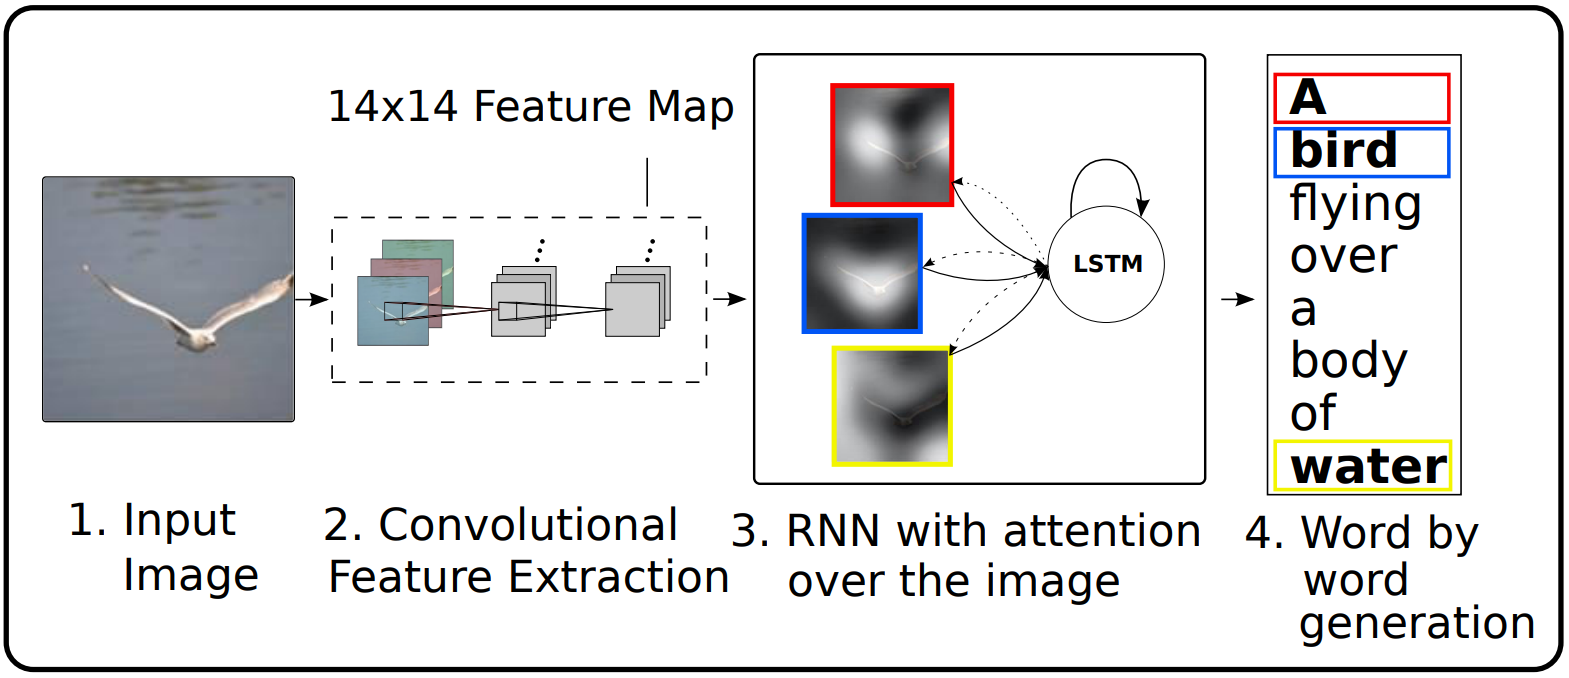
\includegraphics[width=0.7\linewidth]{./img/img_captioning.png}
\caption{
    Diagram of natural language image description using Attention
    (from \cite{ref:img-captioning}).
}
\label{fig:description}
\end{center}
\end{figure}

\subsection{Motivation and Objectives}
In spite of the recent adoption of Attention by a variety of Deep Learning models
and the significant improvements it has shown, we conjecture that there are still many other tasks
that is still not very well explored.
Current works also tend to focus more on the filtering functionality of Attention,
but there are other aspects
-- such as the allocation of mental resources in the course of time -- that can be of potential benefit
(we further discuss the taxonomy of Attention in following sections).
Furthermore, we note that Attention models currently being used
are very specific to each problem in question.
Some works propose a higher level of generalization~\cite{ref:recurr-models},
but we believe it is possible to go further.
Therefore, the specific objectives of this work are:
\begin{itemize}
    \item To perform an extensive literature review on the use of Attention
        in modern Deep Learning;
    \item To identify theoretical aspects of Attention itself from areas such as psychology and neuroscience;
    \item To establish general elements of Attention to be applied to Deep Learning;
    \item To identify specific problems in different classes
        (robotics, vision, natural language, program composition) with
        improvement potential through the use of Attention;
    \item To propose and implement one or more solutions based on the findings of the work to
        validate the ideas and evaluate them in an application.
    %\item To study the viability of generalization of Attention
    %    to broader areas in AI other than Deep Learning.
\end{itemize}

The main contribution of the work proposed is related to the first four items:
we wish to
\emph{establish a theoretical framework of Attention as a series of components
    and its applicabilities to Deep Learning.}
Recent works show that the effort on establishing more general concepts and frameworks for
Deep Learning design has been broadly useful.
Examples include the ideas of \emph{Curriculum Learning}~\cite{ref:curriculum}
and \emph{Generative Adversarial Networks}~\cite{ref:gans}.

\newpage
\section{Background}
\subsection{Attention}
\label{attention}
The interest in the concept of Attention exists since a long time ago.
Throughout the years, Attention has been studied
from various perspectives~\cite{ref:esther-thesis}
such as philosophy, psychology, and neurology.
There are multiple definitions of the concept.
In the next items, we discuss some concrete aspects related to Attention.

\subsubsection{A definition}
\label{sec:attdef}
We can define Attention as
\emph{the act of applying mental resources to selected stimuli following an allocation policy specific to
    a particular goal}.
This rather broad definition captures well the main concepts related to Attention:
in a world with virtually infinite
\emph{stimuli} to select from the environment, agents with otherwise \emph{finite processing
resources} (but with a variety of options of \emph{mental processes} to perform) must choose what their
actions will be (and in which stimuli) in a \emph{correct sequential manner} and in \emph{sensible time}.
As mentioned before, other works may define Attention in a different manner
that is perhaps even conflicting with ours but
these are the terms that we choose our work to be based on -- noting that they
reasonably capture common concepts of interest by us and other works.~\cite{ref:helgason}

\subsubsection{Functionalities of Attention}
Attention can be manifested in different manners depending on the goal.
The most notable functionalities shown in intelligent beings are:
\begin{itemize}
    \item \textbf{To select stimuli} such as looking at only a relevant portion of an image --
        to efficiently use resources on relevant information.
    \item \textbf{To sustain focus} on a specific semantic element for a period to complete
        a task.
    \item \textbf{To guide processing} in a sequential manner that is relevant for a task.
    \item \textbf{To orient resources} to new important stimuli
        -- such as an abrupt noise coming from somewhere --
        or even in alternating the focus to multiple tasks at the same time.
\end{itemize}

\subsubsection{Bottom-up and Top-down Attention}
\label{bu-td}
Focus may emerge in two fundamentally different manners~\cite{ref:esther-thesis}~\cite{ref:vocus}.
In bottom-up Attention, the act of focusing is involuntarily
started and guided by (usually) external and conspicuous stimuli,
such as a shattering glass that tends to
make us immediately turn our heads towards where the noise origin.
Another example is visual saliency (figure \ref{fig:saliency}):
a glowing red ball suddenly appearing in
your field of vision will probably grab your focus.
In top-down Attention, cognition and goals guide voluntarily the focus.
If we are talking to someone in a crowded party, for example,
we focus on what the specific person is saying
-- ignoring other people's words -- to maintain the conversation.

\begin{figure}
\begin{center}
        \begin{tabular} {cc}
        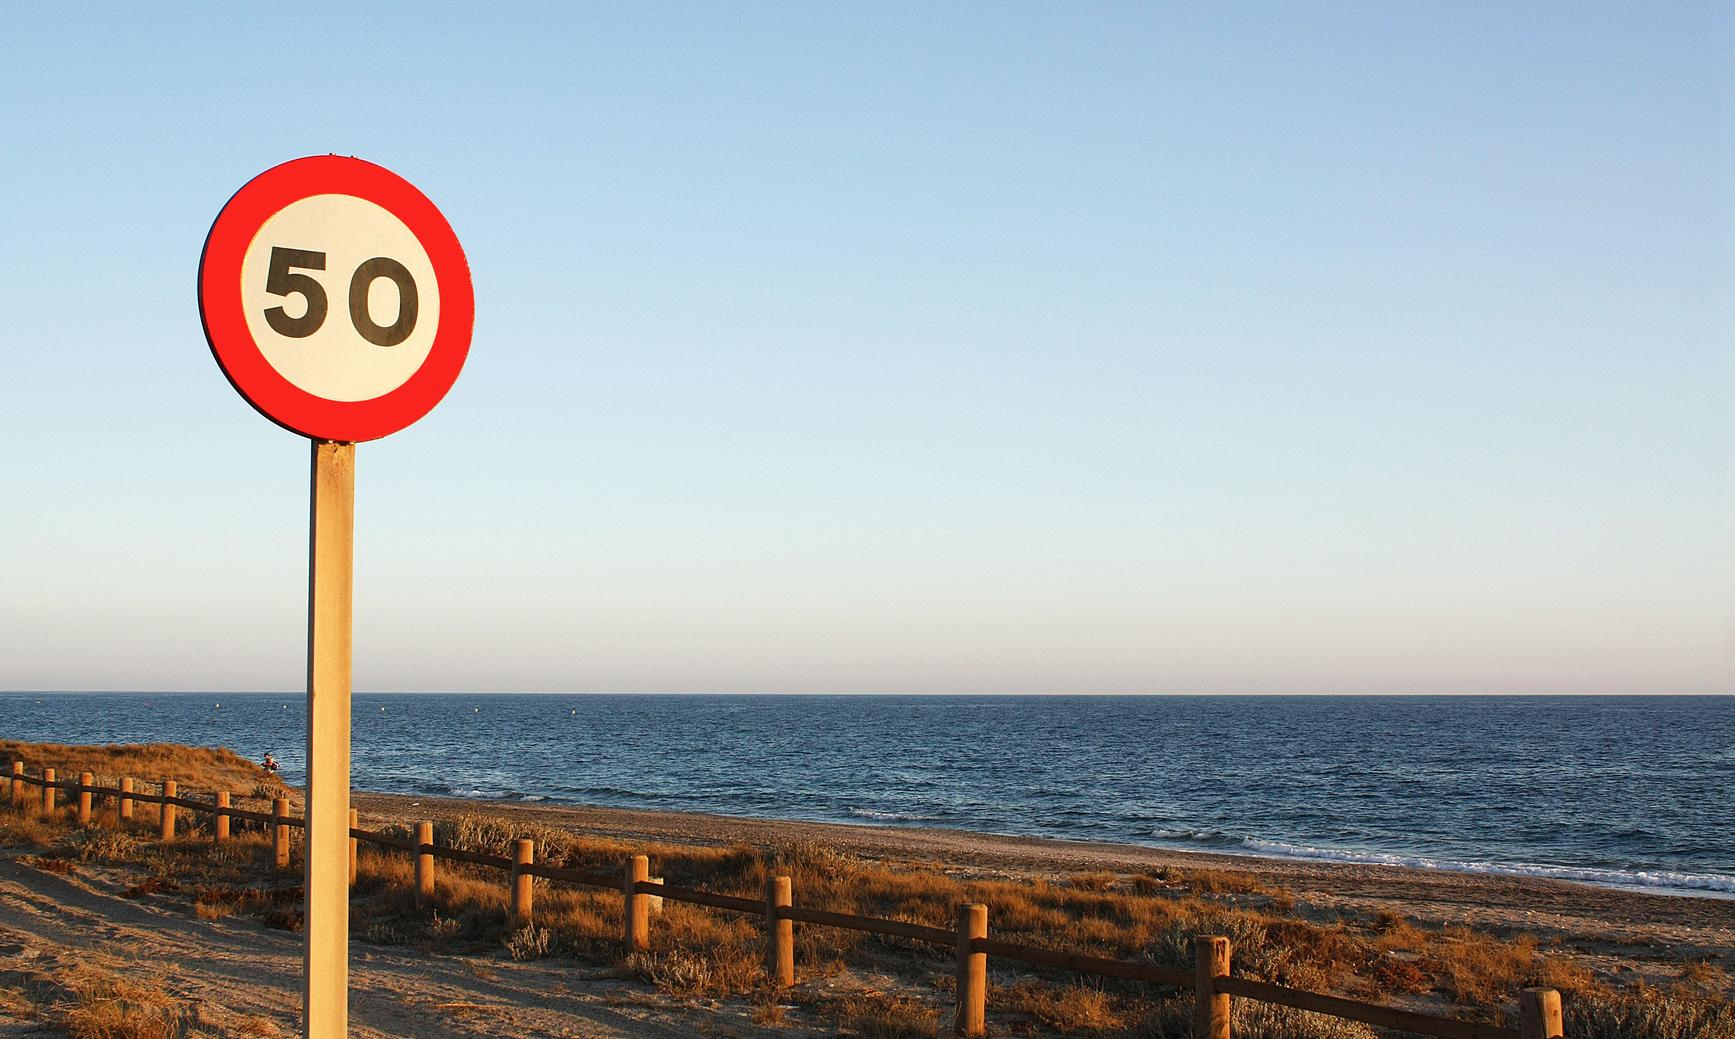
\includegraphics[width=0.35\linewidth]{./img/traffic_sign_s.jpg} &
        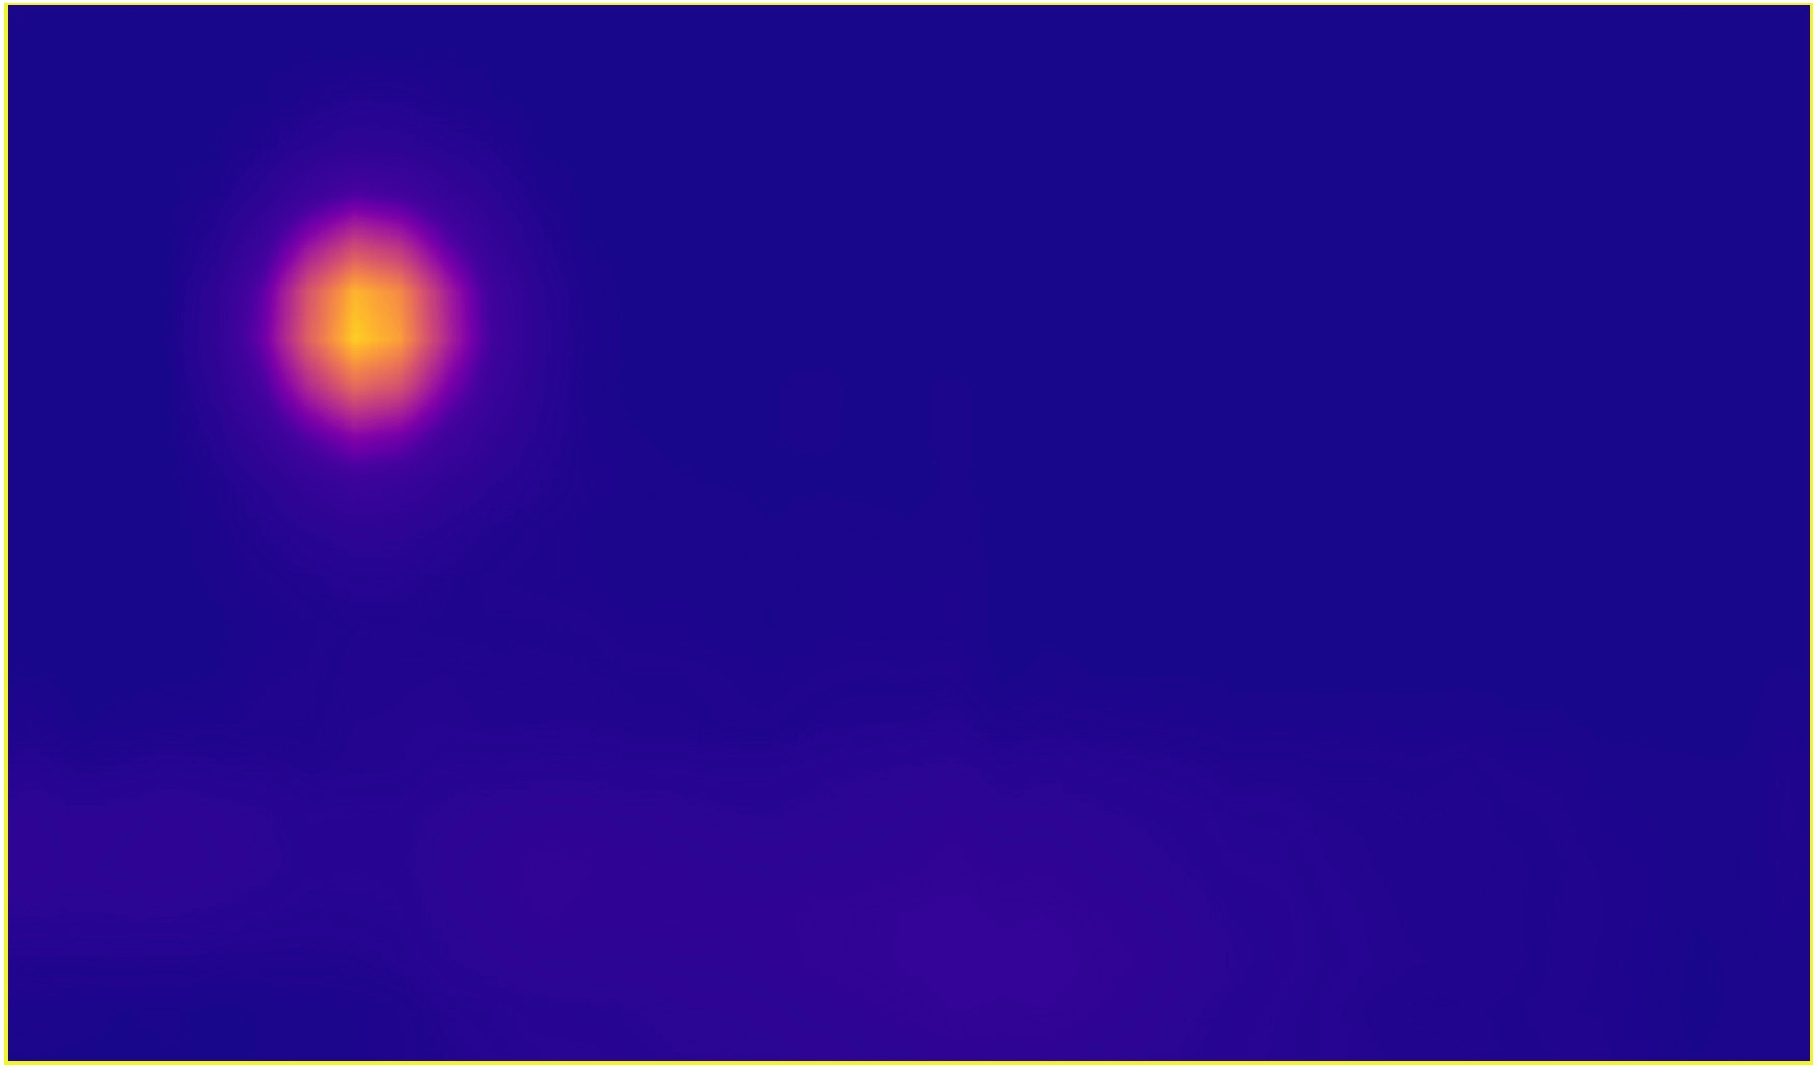
\includegraphics[width=0.35\linewidth]{./img/traffic_sign_m.jpg}\\
        (a) & (b)
        \end{tabular}
\caption{Example of visual saliency.
    b) is the saliency map where higher intensity pixels represent
    regions that are more salient to humans than original image a).}
\label{fig:saliency}
\end{center}
\end{figure}

\subsubsection{Soft and Hard Attention}
In recent years, there has been a useful distinction between
soft and hard Attention~\cite{ref:att-survey}.
Soft Attention regards defining a continuous distribution of importance
across all elements of information for some task.
In the example of visual saliency, one can determine a saliency map $M$
to a given image $I$ where each pixel will have a value in $[0, 1]$
regarding its saliency.
Hard Attention regards determining a discrete subset of
important information elements.
Using the problem of visual saliency again as an example,
one might want to determine a specific location $(i, j)$ of the image
to be used as the center of a small patch of the image that is the most
relevant to be further processed.

\subsection{Deep Learning}
Deep Learning (DL) is a trend in modern AI~\cite{ref:dl}.
Although DL was broadly adopted around 12 years ago,
some of its concepts date to much earlier than that~\cite{ref:dl}:
discussions about the foundations of artificial neural networks go back
to the 1950s, the introduction of backpropagation to the 1970s
and many other key concepts that are popular mostly in the last decade or less
were introduced more than 30 years ago.
Many fields of AI witnessed a significant shift in paradigm
in the last years: models applying DL concepts now achieve state-of-the-art results in different problems regarding Computer Vision,
audio processing, NLP, neural computation among others~\cite{ref:dl-book}.
DL used both in supervised and unsupervised learning~\cite{ref:dl}.

One of the critical concepts of DL is that of the hierarchy of features~\cite{ref:dl}:
A deep sequence of layers apply non-linear transformations to the data
in such a way that many models learn to extract features of hierarchical
levels of abstraction.
For this reason, DL is also regarded as Representation Learning.
This characteristic enables such models to learn the latent structure
in intrinsically unstructured data such as images, text and audio signals.
Another advantage is that of transfer learning: models that are
primarily trained for a given task can be used and adapted for another
task while using at least part of the representations learned.
We discuss some concepts related to DL in following items.

\subsubsection{Artificial Neural Networks}
Artificial Neural Networks (ANNs) are usually adopted to predict
an output by employing learning a non-linear function approximation.
The ideas used in ANNs date to more than 50 years ago~\cite{ref:perceptron} and many of them
are inspired by observed mechanisms of the human brain.
Most of DL models are a variation of one of the families of ANNs
that will be briefly discussed here.

One of the most basic examples is that of Multi-Layer Perceptrons (MLPs).
The main characteristic of this model is the use of hidden layers
and neurons are a linear combination of previous layers followed by
a non-linear activation.
Each layer $l_k$ (with $n$ neurons) is connected to the previous layers
$l_{k-1}$ (with $m$ neurons) and the neuron $l_k^i$, $1 \le i \le n$
is given value:
$$l_k^i = h\left(\sum_{j=1}^{m} l_{k-1}^jw_k^j + b_k^j\right)$$
%Where $h(x): \mathbb{R} \mapsto \mathbb{R}$ is a non-linear activation funcion.
Commonly used activation functions are the sigmoid, hyperbolic tangent
and the Rectified Linear Unit (ReLU):
$$f(x) = \begin{cases}
    0, & x < 0 \\
    x, & x \ge 0 \\
        \end{cases}
$$
ReLU is currently broadly adopted due to its high efficiency
and training speed~\cite{ref:relu}.

\begin{figure}
\begin{center}
    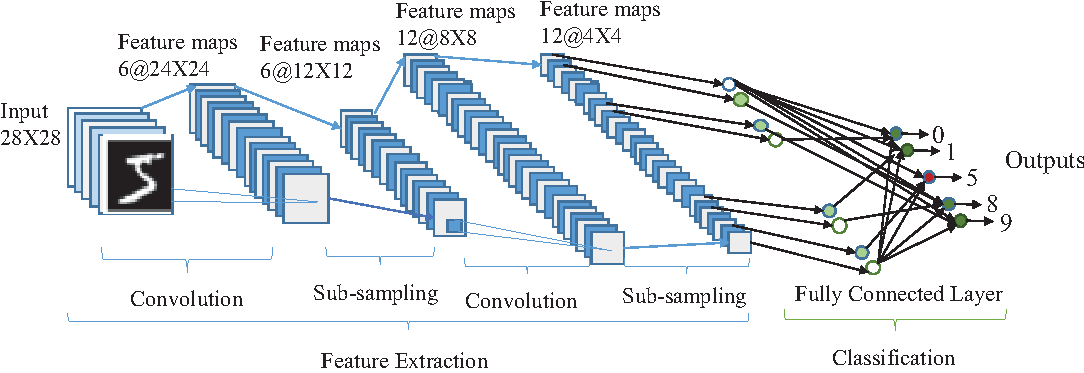
\includegraphics[width=0.9\linewidth]{./img/cnn2.png}
\caption{
    Diagram of a convolutional neural network.
    Learned filters extract features in an increasingly hierarchical manner.
}
\label{fig:cnn}
\end{center}
\end{figure}

\subsubsection{Convolutional Neural Networks}
Convolutional Neural Networks (CNNs) are widely used in Computer Vision tasks such as image classification, localization, and semantic segmentation.
CNNs use the fact that images tend to have correlated pixels and use
convolution filters in an hierarchical manner (figure \ref{fig:cnn})
to learn features in increasing abstraction.
For a certain layer, the $i$-th feature map $m_i$ is,
given filter weights $W_i$, bias $b_i$ and nonlinearity function $h(x)$,
obtained as:
$$m_i = h\left(W_i * x + b_i\right)$$
with $*$ as the convolution operation.

\begin{figure}
\begin{center}
    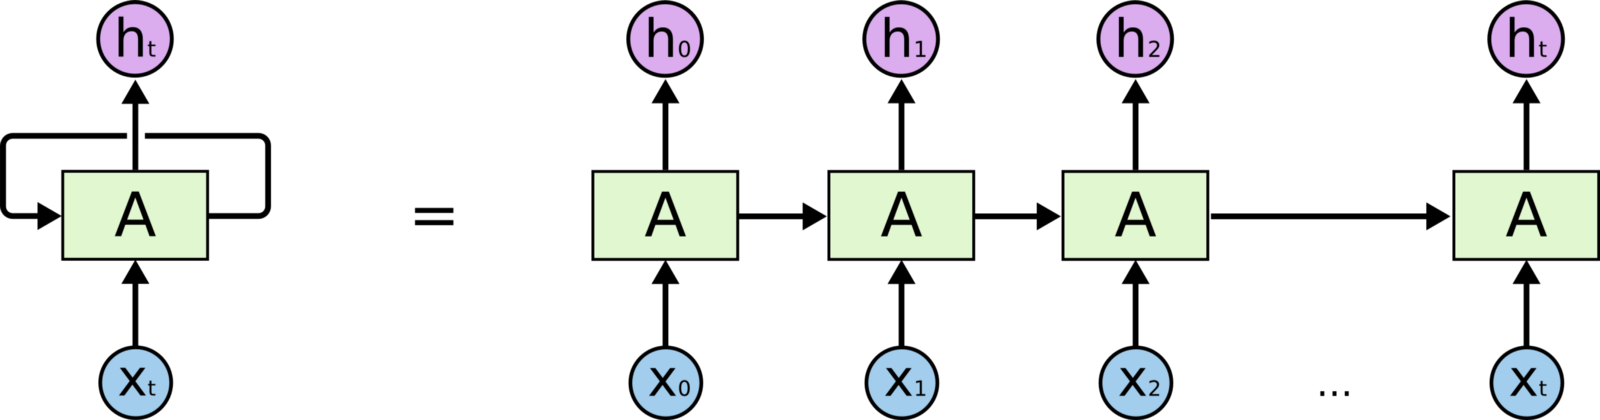
\includegraphics[width=0.9\linewidth]{./img/rnn2.png}
\caption{
    Diagram of a recurrent neural network.
    Time steps map previous outputs and current input to another time step.
}
\label{fig:rnn}
\end{center}
\end{figure}

\subsubsection{Recurrent Neural Networks}
A recursive architecture characterizes recurrent Neural Networks (RNNs)
that uses the input of the current step and the output of the previous
step to compute the predictions.
The hidden state $h_t$ at time step $t$, given input $x_t$, weight matrix $W$,
previous state $h_{t-1}$, hidden-state-to-hidden-state matrix $U$ and
non-linearity $f(x)$ is given by:
$$h_t = f\left(Wx_t + Uh_{t-1}\right)$$
These architectures are widely used in NLP tasks such as
machine translation~\cite{ref:rnn-nlp}.
Some variations over the original basic architecture such as
LSTMs are also broadly adopted.

\textbf{Modern architectures}
Modern work on Deep Learning propose models of greater complexity than cited above.
Some present completely novice architectures, but most of the work are a combination of basic neural networks architectures. The final results, however, may consist
of entirely new contributions to new tasks.
Some examples will be discussed in section \ref{sess:related-work}.

\subsubsection{Learning process}
The act of learning the appropriate weights of a given model
is usually obtained by the minimization of a differentiable loss function
that is the cost function $L(y, \hat{y})$ that characterizes the error
between the true value $y$ and the predicted value $\hat{y}$.
Backpropagation~\cite{ref:backprop} plays an essential role in DL because it is used to adjust the weights $\theta$ of models that have a
differentiable cost function.
A typical training process is composed of a forward-propagation
step which computes the predictions over a set of input samples
and a backpropagation step which calculates the loss function
and adjusts the weights of the model.
In DL, common adjustment methods includes Gradient Descent (GD)~\cite{ref:gd} or variations
which, for a given minibatch, adjusts weights according to:
$$\theta_{i+1} = \theta_i - \alpha\frac{\partial{J}}{\partial{\theta}}$$
where $\alpha$ is the learning rate.

\vspace{2cm}
\section{Related Work} \label{sess:related-work}
The topic of integrating Attention concepts into Deep Learning has been increasingly frequent
in the community~\cite{ref:att-survey}.
Augmenting the capabilities of neural network architectures with Attention has shown promising results
in problems from a variety of fields in which Deep Learning is currently being applied to, such as
Computer Vision, Natural Language Processing and differentiable programming in general.
In this subsection, we address some recent works.
We highlight how The authors used attention and how it affected the performance of the proposed models
on evaluation tasks.

\subsection{Attention-based Encoder-Decoder Networks}
Encoder-decoder networks are a general framework generally used for mapping from input to outputs that both
are of highly-dimensional (often unstructured) data, having been successfully used for tasks such
as machine translation~\cite{ref:enc-dec-rnns}.
One drawback of such architecture is that the encoded feature vector is of fixed size and structure --
regardless of the input -- and not necessarily preserves spatial/temporal structure from the data.
The work in \cite{ref:enc-dec} proposes the usage of an attentional module in between encoder and decoder.
The proposed model's encoder produces feature vectors that have an explicit spatiotemporal structure
(\emph{context set}) of the input and the attentional module uses a relevance evaluation
method to select a subset of the outputs -- either by soft Attention or hard Attention.
This allows the encoder-decoder for more flexibility to select the components of the input that is of
more relevance.
The authors implemented and evaluated the method for several applications:
\begin{itemize}
    \item \emph{Image Caption Generation}: The goal of the task is to provide a natural language description
        of an input image.
        The proposed model uses a CNN as encoder and RNN as decoder -- with the attentional model in between.
        The model was ranked third in \emph{MS COCO Captioning Challenge} and provided highly interpretable
        results regarding the importance of the regions of the image to each component of the sentence
        (see figure \ref{fig:description}).
    \item \emph{Neural Machine Translation}: The authors proposed an RNN architecture augmented with the Attention module, which provided a relative improvement of roughly 60\% when compared to the same model without Attention.
        The model also performs better than state of the art in some languages.
        It was also possible to obtain a weight matrix that maps the importance of input to output words since the context set provides structural information of the input (see figure \ref{fig:ntatt}).
    \item \emph{Neural Speech Recognition}: The goal of the task is to translate audio to text sentences by
        using fully neural networks.
        The proposed model uses RNNs between the Attention module and the model achieved state-of-the-art results in the TIMIT corpus~\cite{ref:timit} and the outputs provide Attention weights from
        the input signal to produced phonemes.
\end{itemize}
Overall, the proposed technique -- besides achieving state of the art results --
produces a semantic mapping from the input space to the output space even when they are of different nature
-- without explicitly being supervised to produce this mapping.

\begin{figure}
\begin{center}
    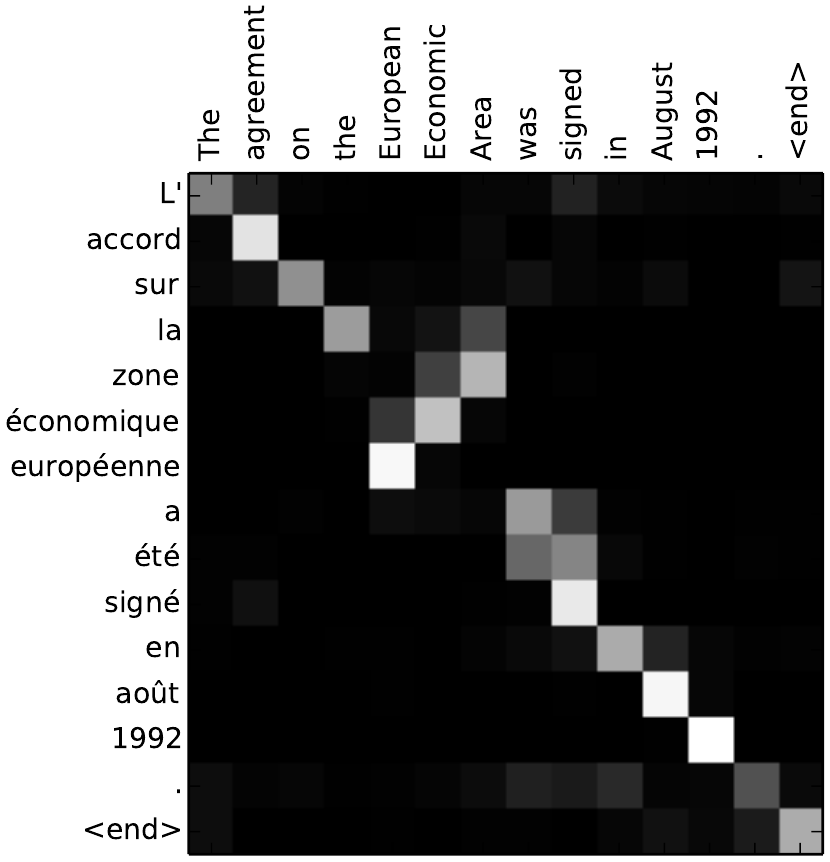
\includegraphics[width=0.31\linewidth]{./img/nt-att.png}
\caption{
    Visualization of Attention weights of the neural machine translation model
    based on Encoder-Decoder networks.
    Figure from \cite{ref:enc-dec}.
}
\label{fig:ntatt}
\end{center}
\end{figure}

\subsection{Adaptive computation time for RNNs}
Most of the current work uses Attention as a mechanism for filtering.
The authors of the work in \cite{ref:act} propose an RNN augmented with an Attention module that allows the dynamic inference of many computation steps for each time step.
It uses soft Attention to determine when to stop (see figure~\ref{fig:adaptive-comp}).
The ability to allocate computational resources is an essential function of Attention.
The authors show that the mechanism allowed for the model to achieve considerably superior results
in tasks such as adding and sorting (when compared to a model without adaptive computation time)
because the model was enabled to perform more or fewer operations depending on nature dynamically
of each step.
The authors also tested the model in the problem of character prediction on the Hutter prize Wikipedia
dataset~\cite{ref:hutter}, in which the model yielded insights into the structure of the input data.

\begin{figure}
\begin{center}
    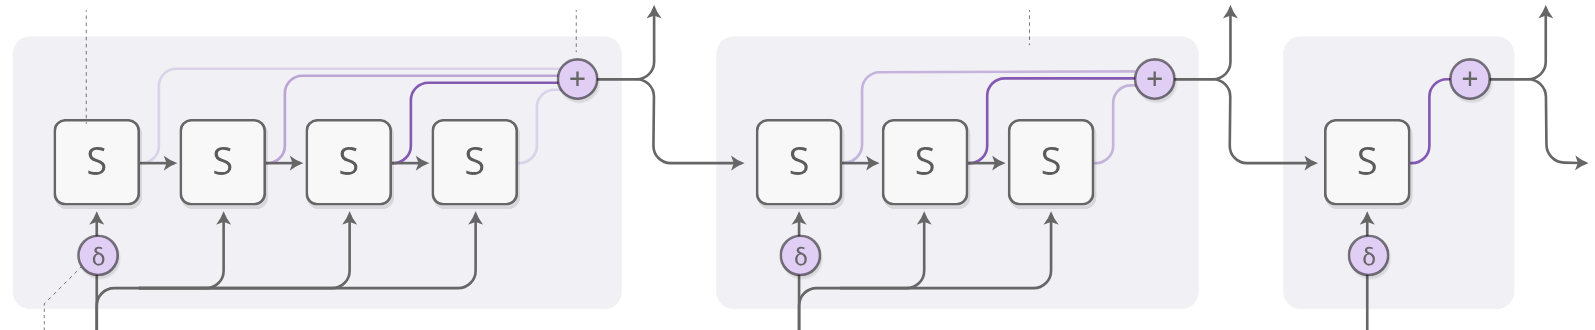
\includegraphics[width=0.9\linewidth]{./img/adaptive_comp.png}
\caption{
    Diagram of the adaptive RNN.
    Each time step can have the number of computations varied by an Attention distribution.
    Figure from~\cite{ref:distill}.
}
\label{fig:adaptive-comp}
\end{center}
\end{figure}

\subsection{Neural Turing Machines (NTMs)}
Neural Turing Machines~\cite{ref:ntm} is one of the first attempts at building models that can learn to
formulate programs based on DL architectures with continuous cost functions
-- and thus trainable via gradient descent.
The proposed model is composed of an RNN connected to an external memory bank -- which can be read/modified
by the use of reading/write heads in the model.
The Attention mechanism is the component that allows for the read and writes operations to be differentiable.
On every read/write step, there is an Attention distribution
-- which is updated each step via content-based and location-based methods --
that operates on vectors in the memory locations in a continuous manner.
The authors show that the model can learn simple algorithms such as sorting and copying sequences.

\begin{figure}
\begin{center}
    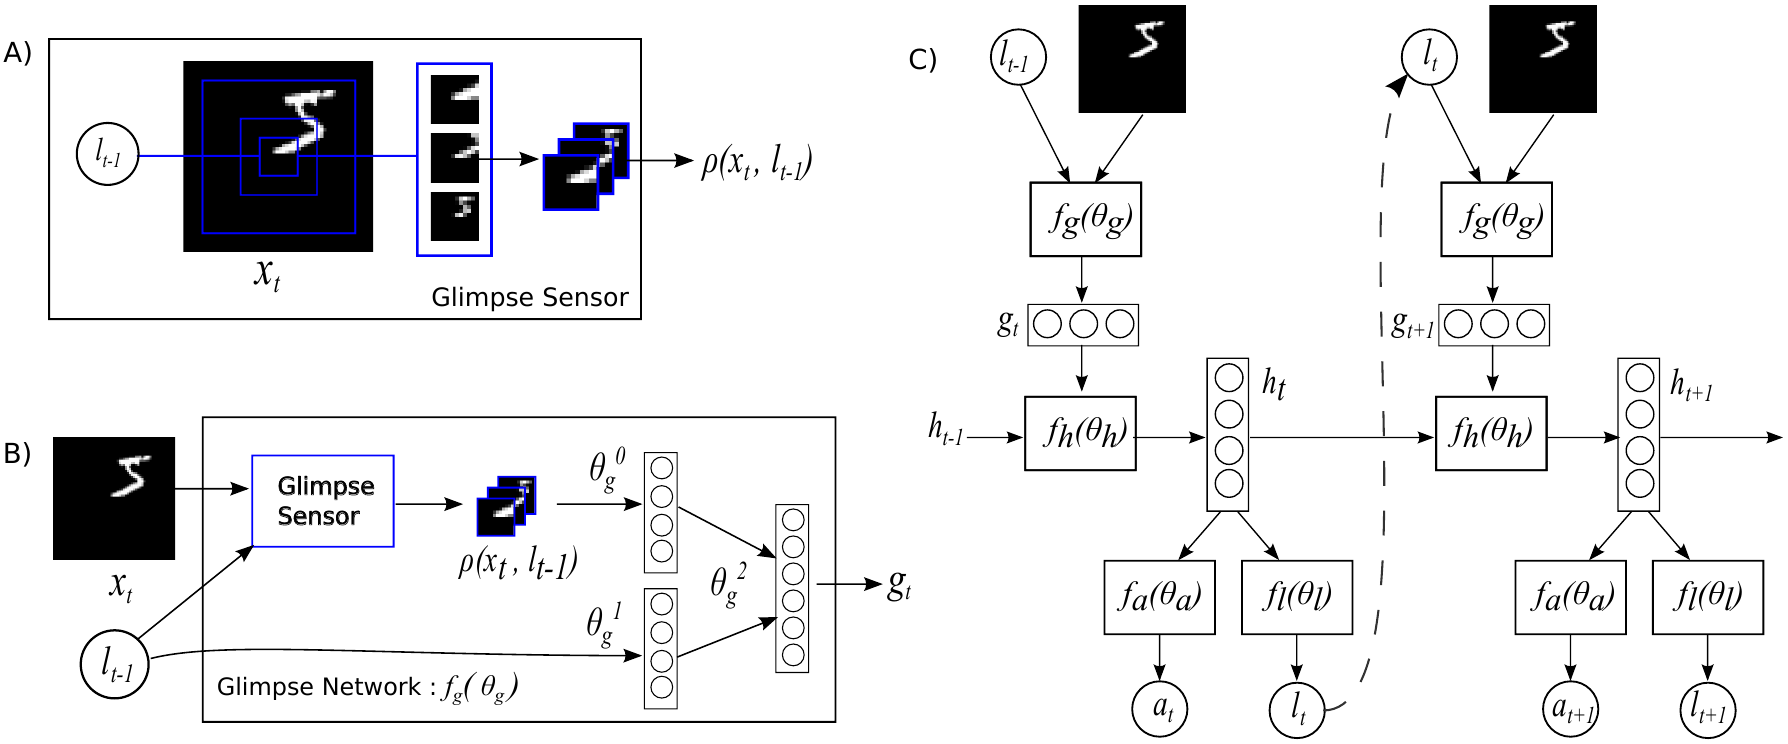
\includegraphics[width=1.0\linewidth]{./img/recurr_model.png}
\caption{
    Overall architecture of the recurrent attentive model.
    \textbf{A)} is the \emph{glimpse sensor} that extracts patches of different resolutions from image
    according to the location being attended.
    \textbf{B)} is the \emph{glimpse module}, which combines information from previous attended locations
    and glimpses to encode a hidden state.
    \textbf{C)} is the RNN architecture augmented with the glimpse module.
    Figure from \cite{ref:rec-models}.
}
\label{fig:recurr-model}
\end{center}
\end{figure}

\subsection{Recurrent Attention Model (RAM)}
The work \cite{ref:rec-models} considers a commonly known problem in Computer Vision: it is usually
expensive to perform processing on images and widely used current models such as
CNNs tend to require computational resources proportional to the number of pixels in the image.
The work proposes a \emph{Recurrent Attention Model (RAM)}, a recurrent neural network augmented by
an attentional component regarded as \emph{Glimpse Module} that is trained via Reinforcement Learning.
The Glimpse Module enables the network to select a point in the image from which it extracts `'glimpses''
-- patches of the image at different resolutions but with the same dimensions.
These glimpses and the selected location are encoded and given as input to produce
the new hidden state of the core RNN architecture (see figure \ref{fig:recurr-model}).
The dimensionality of the glimpse is much smaller than that of the image and furthermore does not depend
on the dimensions of the input image.
The authors evaluate the model for classification tasks in the MNIST~\cite{ref:mnist} dataset and variations
in which the input images are filled more background pixels (resulting in a larger image) and clutter.
The proposed model outperforms a convolutional neural network baseline.
Furthermore, the attentional module in the model enables it to perform the same amount of computation
regardless of the input size of the image and to focus sequentially only at the relevant parts of the image,
which reduces the adversary effect of clutter.

\subsection{Neural Programmer}
Deep Learning techniques have been useful for perception tasks in the last years, but tasks that involve
complex logic and reasoning are still a major challenge.
Authors in \cite{ref:np} propose a model that learns to induce programs by composing basic logic operations
into more complex ones in sequence (figure \ref{fig:np}).
The model is differentiable and thus trainable via gradient descent because the authors use an Attention
distribution at each step to select the operations to be used.
The authors of the work evaluate the model on a synthetic table-comprehension dataset.
The model achieved nearly perfect accuracy and yielded superior performance compared to LSTMs.

\begin{figure}
\begin{center}
    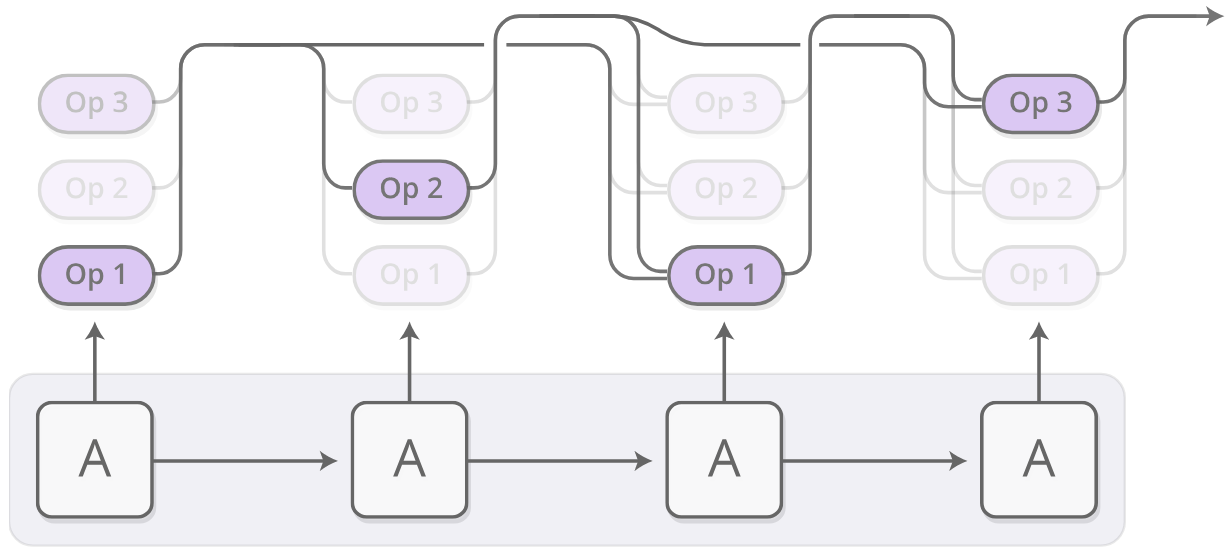
\includegraphics[width=0.5\linewidth]{./img/neural-programmer.png}
\caption{
    Sequence of operations being carried out by the Neural Programmer model.
    Attention distributes the weights to each operation.
    Figure from \cite{ref:distill}.
}
\label{fig:np}
\end{center}
\end{figure}

\subsection{The Transformer architecture}
For sequence modeling tasks such
as machine translation, there is a massive use of sequence models such as RNNs and more specifically LSTMs.
The work proposed in \cite{ref:transformer} aims at overcoming some challenges inherent to such sequential
models, such as performance and obstacles to applying parallelization to the process.
Complications also arise when the content of the inputs are long (such as long sentences in the text) and
recurrent models present difficulties in establishing relationships between words.
The authors present the \emph{Transformer}, an encoder-decoder feed-forward architecture with Attention as a critical element.
The input sentences are embedded, and positional encoding is applied.
Then, each layer of the transformer and the decoder employ either \emph{scaled dot-product Attention} or
\emph{multi-head Attention}, which allows for contextual mapping and representation of long-relationships.
The proposed model achieved state of the art results on \emph{WMT 2014 English-to-German} and
\emph{WMT 2014 English-to-French} translation tasks.

\begin{figure}
\begin{center}
    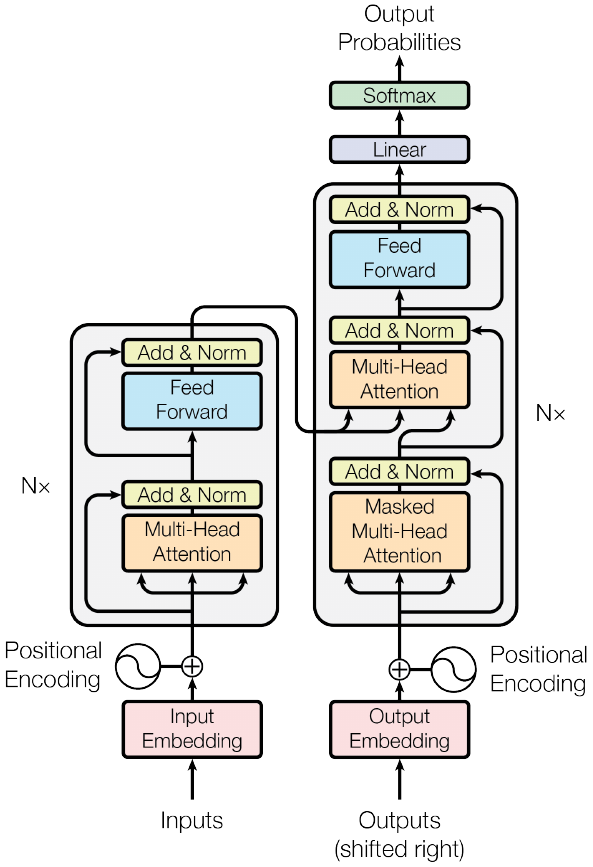
\includegraphics[width=0.4\linewidth]{./img/transformer.png}
\caption{
    The transformer architecture.
    Figure from \cite{ref:transformer}.
}
\label{fig:transformer}
\end{center}
\end{figure}

\let\clearpage\relax

\section{Methodology}
\subsection{Activities}
\label{sec:activities}
The work can be summarized in three main activities (or \textbf{phases}):
\begin{itemize}
    \item \textbf{1. Literature Review}: an extensive survey on current uses of Attention in modern
        Deep Learning.
    \item \textbf{2. Proposal of an Attention framework for Deep Learning}: \
        defining a component set of Attention elements currently used in Deep Learning design from results of previous phase and further survey.
    \item \textbf{3. Implementation of Attention in Deep Learning}:
        proposing of one or more models with components of Attention and evaluations on a set of tasks.
\end{itemize}

More specifically, the activities to be executed are:

\begin{itemize}
    \item \textbf{A1.1 - Theoretical definition of Attention and its components:}
        From a variety of previous works~\cite{ref:helgason}\cite{ref:esther-thesis},
        we establish a theoretical framework of Attention
        -- extending what was discussed in subsection \ref{attention} --
        on which all later work will be based.
        It is worth noting that this theoretical framework is not necessarily the same as the framework
        we propose to produce specifically for Deep Learning in phase 2.

    \item \textbf{A1.2 - Elaboration of survey:}
        Exploration of selected work under the point of view of the theoretical framework established
        in \textbf{A1.1}.
        For each work, we identify the main components of Attention the authors use, the consequences for the
        performance in the application domain and elaborate a critical evaluation.

    \item \textbf{A1.3 - Survey article writing:}
        Writing of an article with results of phase $2$ to be sent to an appropriate journal.

    \item \textbf{A2.1 - Establishment of Attention components for specific Deep Learning domains:}
        From the theoretical framework obtained in \textbf{A1.1}
        and the exploration of current uses and results in \textbf{A1.2},
        we devise sets of useful components of Attention for specific main problem domains
        in which Deep Learning is broadly used,
        such as image classification, text-to-speech, language translation, image segmentation.

    \item \textbf{A2.2 - Establishment of Attention framework for Deep Learning:}
        From the theoretical framework obtained in \textbf{A1.1},
        exploration of current uses and results in \textbf{A1.2} and
        results from \textbf{A2.1},
        we elaborate a set of components of Attention under a single framework to be applied to more
        general areas of use of Deep Learning,
        such as Computer Vision, Sequence Processing, Program Composition.

    \item \textbf{A3.1 - Arrangement of experiments:}
        From the framework obtained in phase 2, we select a set of problem domains (such as text-to-speech),
        Deep Learning models to use, components of Attention to implement and metrics to evaluate the task.
        The activity aims at selecting all main devised components from phase $2$ in order
        to evaluate the real consequences of their adoption against what was predicted.

    \item \textbf{A3.2 - Execution of experiments:}
        We implement and execute the planned experiments following a pre-defined protocol that
        pays particular attention to reproducibility.

    \item \textbf{A3.3 - Evaluation of experimental results:}
        We evaluate the results using established metrics for each experiment,
        elaborating discussions that include exciting aspects of the results in general and
        comparisons between the theoretical predictions and the concrete outcomes.
        It is worth noting that the metrics we'll use will vary depending on the specific problem,
        but they will always be selected so as to reflect the improvement of the models with the use of
        attention.

    \item \textbf{A3.4 - Experiments article writing:}
        Writing of an article with results of phase $3$ to be sent to an appropriate conference.
\end{itemize}

Other activities to be done related to the masters program are:
\begin{itemize}
    \item \textbf{A0.1 - Course's requirement fulfillment.}
    \item \textbf{A0.2 - Qualification Exam.}
    \item \textbf{A0.3 - Masters dissertation.}
    \item \textbf{A0.4 - Defense of masters dissertation.}
\end{itemize}

\subsubsection{Schedule}
Table~\ref{table:sched} details the project schedule.
Considering the start of the program in the second semester of 2018, the duration of the work is expected to be
one and a half years.

\begin{table}[H]
\centering
\caption{\small Project schedule.}
\scriptsize
\begin{tabular}{|c|c|c|c|c|c|c|c|c|c|c|c|c|c|c|c|}
	\hline
    \multirow{2}{*}{\textbf{Activity}}
        & \multicolumn{3}{|c|}{\textbf{2018}} & \multicolumn{12}{|c|}{\textbf{2019}}\\
    \cline{2-16}
                  & Oct & Nov & Dec & Jan & Feb & Mar & Apr & May & Jun & Jul & Aug & Sep & Oct & Nov & Dec\\
    \hline
    \textbf{A0.1} & $*$ & $*$ & $*$ &     &     &     &     &     &     &     &     &     &     &     &     \\
    \hline
    \textbf{A1.1} & $*$ &     &     &     &     &     &     &     &     &     &     &     &     &     &     \\
    \hline
    \textbf{A1.2} &     &     &     & $*$ & $*$ & $*$ & $*$ & $*$ & $*$ & $*$ &     &     &     &     &     \\
    \hline
    \textbf{A0.2} &     &     &     &     &     &     &     & $*$ &     &     &     &     &     &     &     \\
    \hline
    \textbf{A1.3} &     &     &     &     &     &     &     &     &     & $*$ &     &     &     &     &     \\
    \hline
    \textbf{A2.1} &     &     &     &     &     &     &     &     &     & $*$ &     &     &     &     &     \\
    \hline
    \textbf{A2.2} &     &     &     &     &     &     &     &     &     &     & $*$ &     &     &     &     \\
    \hline
    \textbf{A3.1} &     &     &     &     &     &     &     &     &     &     & $*$ &     &     &     &     \\
    \hline
    \textbf{A3.2} &     &     &     &     &     &     &     &     &     &     & $*$ & $*$ & $*$ & $*$ &     \\
    \hline
    \textbf{A3.3} &     &     &     &     &     &     &     &     &     &     &     &     &     & $*$ &     \\
    \hline
    \textbf{A3.4} &     &     &     &     &     &     &     &     &     &     &     &     &     & $*$ &     \\
    \hline
    \textbf{A0.3} &     &     &     &     &     &     &     &     &     &     &     &     & $*$ & $*$ & $*$ \\
    \hline
    \textbf{A0.4} &     &     &     &     &     &     &     &     &     &     &     &     &     &     & $*$ \\
    \hline
\end{tabular}
\label{table:sched}
\end{table}


\section{Preliminary Work}
In this section we briefly describe the results of the activities performed so far.

\subsection{Theoretical Definition of Attention}
Activity \textbf{A0.1} (described in~\ref{sec:activities}) was successfully completed,
resulting in a theoretical framework for attention upon which we can build future work.
This task is very important since we want to be as clear as possible regarding what we define as ``attention''.
In the framework, we define a set of \emph{entities of interest} and the phenomenon of Attention in terms of
its \emph{functionalities} and how it relates to the entities.
An initial definition was given in~\ref{sec:attdef} -- we used part of it as a basis for the complete framework.

\subsubsection{Why is our framework good?}
We believe our framework encompasses what we generally (and intuitively) refer to as attention while being not too broad.
Also, the definition is given in terms related to Computer Science so it’s functionality nicely translates to the domain,
which is important since we (so far) intend to develop AI using computers as we know it today.
Our definitions may not encompass every aspect of Attention and even be conflicting with other definitions.
However, this is the set of postulates that we think is the most precise and useful and thus this is
what we choose to use for future work to be based on.

\subsubsection{Entities}
Below is the list of entities - or “terms” - we use in this work, along with a brief discussion of the meaning
we give to each term in the context of this work.

\begin{itemize}
    \item\textbf{Data:} information, stimuli. It may be internal or external. Examples: visual information, audio, memories.
    \item\textbf{Program:} algorithm, sequence of computer (or mental) operations. Programs use data as input in order to carry out a sequence of operations that produces output data and/or actions.
    \item\textbf{Process:} the execution of a program on a specific data instance.
    \item\textbf{Computer:} the executor of processes, the “brain”.
    \item\textbf{Resource:} when not specified, we mean “computational resources”, e.g. CPU time.
    \item\textbf{Time:} the flow of time.
    \item\textbf{World:} the external environment.
    \item\textbf{Agent:} the actor in the world.
    \item\textbf{Actions:} the interaction of the agent with the world.
    \item\textbf{Goals:} the ends, objectives to be met.
\end{itemize}

\subsubsection{A broad definition of Attention}
\emph{Data}, \emph{programs} and \emph{processes} are virtually \emph{infinite}.
Computational \emph{resources} and \emph{actions} are finite.
\emph{Attention} is \emph{the system of allocating resources to processes}.
In other words, \emph{attention} is the entity in \emph{agents} that, given \emph{context} and a set of \emph{processes},
\emph{allocates} \emph{resources} to execute each of them in order to \emph{produce} \emph{outputs} in form of \emph{data} and \emph{actions} in a \emph{correct sequential manner} and in \emph{sensible time} in order to reach \emph{goals}.


\subsubsection{Taxonomy of Attention}
We classify attention in terms of its functionalities, e.g. what it does.

\textbf{Classification Dimensions}: Attention can be seen in terms of the type of actions it executes,
the targets of these actions in the agent, the continuity of the action and the time signature of the action.
In agents, the actions may be initiated from the agent itself (top-down) or be triggered from the world (bottom-up).

Some examples of actions attentional systems perform:
\begin{itemize}
    \item weighting of stimulus (e.g. visual saliency)
    \item selection of items to be processed later
    \item allocation of computing time to a certain processing routine from a “budget”
\end{itemize}

In all these actions, the underlying principle is that of allocating resources to processes.
This allocation can be seen as a form of selection over the three variables attention is concerned: data, programs, resources.
The amount of resources may be fixed while the process varies (as in visual saliency) or the input and program may be fixed
while the amount of resources varies (as in the example of adaptive computation time in RNNs).
The three variables might vary as well.
The taxonomy can be summarized as follows:

\begin{itemize}
    \item \textbf{Actions}:
    \begin{itemize}
        \item Selection
    \end{itemize}

    \item \textbf{Targets}:
    \begin{itemize}
        \item Data
        \begin{itemize}
            \item Item-wise
            \item Location-wise
            \item Feature-wise
        \end{itemize}
        \item Program
        \item Resources
    \end{itemize}

    \item \textbf{Continuity}:
    \begin{itemize}
        \item Soft
        \item Hard
    \end{itemize}

    \item \textbf{Time signature}:
    \begin{itemize}
        \item One to one
        \item One to many
        \item Many to one
        \item Many to many
    \end{itemize}

    \item \textbf{Action initiator}:
    \begin{itemize}
        \item Internal (top-down)
        \item External (bottom-up)
    \end{itemize}
\end{itemize}

\subsection{Survey}
Activity \textbf{A1.2} (described in~\ref{sec:activities}) is currently in progress.
We now report the progress made so far.

\subsubsection{Collection of relevant works}
The first step was to search in the literature for works which applied some form
of ``attention'' to Deep Learning.
A methodology for searching and selecting the works was established,
which we summarize below:

\begin{itemize}
    \item \textbf{Publication date range}: from 2014 to 2019
    \item \textbf{Databases searched}:
    \begin{itemize}
        \item \textbf{arXiv} - \texttt{https://arxiv.org/}
        \item \textbf{DeepMind} - \texttt{https://deepmind.com/research/publications/}
        \item \textbf{Google AI} - \texttt{https://ai.google/research/pubs/}
        \item \textbf{OpenAI} - \texttt{https://openai.com/research/#publications}
        \item \textbf{Facebook AI research} - \texttt{https://research.fb.com/publications/}
        \item \textbf{Microsoft research} - \texttt{https://www.microsoft.com/en-us/research/search/}
        \item \textbf{Amazon research} - \texttt{https://www.aboutamazon.com/publications}
        \item \textbf{Google Scholar} - \texttt{https://scholar.google.com.br/}
        \item \textbf{IEEE Xplore} - \texttt{https://ieeexplore.ieee.org/Xplore/home.jsp}
        \item \textbf{DBLP} - \texttt{https://dblp1.uni-trier.de}
        \item \textbf{ACM} - \texttt{https://dl.acm.org/}
        \item \textbf{NIPS} - \texttt{https://nips.cc/}
        \item \textbf{ICML} - \texttt{https://icml.cc/}
        \item \textbf{ICLR} - \texttt{https://iclr.cc/}
        \item \textbf{AAAI} - \texttt{http://www.aaai.org/}
        \item \textbf{CVPR} - \texttt{http://cvpr2018.thecvf.com/}
        \item \textbf{ICCV} - \texttt{http://iccv2017.thecvf.com/}
        \item \textbf{CoRR} - \texttt{https://arxiv.org/corr/home}
        \item \textbf{Neurocomputing} - \texttt{https://www.journals.elsevier.com/neurocomputing}
    \end{itemize}
    \item \textbf{Terms (in title or abstract)}:
    \begin{itemize}
        \item attention
        \item attentive
        \item attentional
    \end{itemize}
\end{itemize}

The relevance of each work was confirmed upon reading of the abstract.
As a result, we collected around 300 papers.

\subsubsection{Literature Visualizations}
Some visualizations were generated for the works collected with the intent
to have some insights regarding the collection acquired.
Some visualizations generated were:
\begin{itemize}
    \item Citations graph (authors and works)
    \item Abstract/title word frequencies
    \item Frequency of attention-themed papers over years
    \item Relative Frequency of attention-themed papers over years for some databases (arXiv, CVPR, DBLP)
\end{itemize}
Visualizations were generated by a set of scripts which can be found at \url{https://github.com/erikperillo/litrev}.

\subsubsection{Paper relevance analysis}
With the collection in hands, the next goal was to assess the relevance and problem domain of each work
via a paper relevance analysis~\cite{ref:paper-relevance}.
To each work, we attributed the citation count, domains (e.g. Computer Vision), subdomains (e.g. image classification)
and an ``impact'' score ranging from 1 to 5. This score was assessed in a quick and rough manner via the abstract of each
work and it was given based on criteria such as:
\begin{itemize}
    \item How innovative is the proposed model(s) of the work?
    \item How general is the proposed model(s)?
    \item Does the proposed model(s) achives/surpasses state-of-the-art in some task?
    \item Is attention a central component to the results of the work?
\end{itemize}

\subsubsection{Reading and summarization of works}
This step (which is in progress) aims at reading each paper of the collection in depth (in order of relevance, from highest to lowest) and generating a summary for each work.
A summary template was formulated~\cite{ref:paper-anal-template} and summaries were generated for some works.
This is the main step of the survey and it's expected to be the longest.
The goal is to further refine our theoretical framework and guide the reading of future papers as we read those papers
-- in an iterative manner.

%\renewcommand\bibname{References\vspace*{10mm}}
\newpage
\printbibliography

%\begingroup
%\let\clearpage\relax
%\bibliographystyle{plain}
%\bibliography{proposal.bib}
%\printbibliography
%\endgroup

\end{document}
